\documentclass[11pt]{article}

% Packages
\usepackage[utf8]{inputenc}   % For UTF-8 encoding
\usepackage{amsmath, amssymb} % For mathematical symbols
\usepackage{graphicx}         % For including graphics
\usepackage{geometry}         % For adjusting page dimensions
\usepackage{hyperref}         % For hyperlinks
\usepackage{booktabs}         % For nicer tables
\usepackage{float}            % For figure placement

% Page layout
\geometry{a4paper, margin=1in}

% Document Info
\title{Final Project Status Report}
\author{Yijia Zhou}
\date{\today}

% Begin Document
\begin{document}

\maketitle


\section{Introduction}
Open Source Energy Modeling System (OSeMOSYS) is an open-source energy modeling system that provides a framework for simulating and optimizing energy systems. It is designed to be flexible and extensible, allowing users to model a wide range of energy technologies and systems. The main goal of OSeMOSYS is to support decision-making in energy planning and policy by providing insights into the costs, emissions, and other impacts of different energy scenarios. Based on the design and development of the OSeMOSYS model \cite{Howells2011}, this project aims to enhance and improve the original open source model by incorporating additional features and functionalities. The project will involve a comprehensive review of the existing model, identification of areas for improvement, and implementation of new features to enhance its capabilities. The final deliverable will be an updated version of the OSeMOSYS model that is more robust, user-friendly, and capable of addressing a wider range of energy modeling scenarios.

\section{Background}
\subsection{Objectives}
The main objective is to minimize the total Net Present Value (NPV) of the energy system over the entire planning horizon, which includes both investment costs and operational costs. The model aims to achieve this objective while satisfying a set of constraints related to energy demand, resource availability, and technology characteristics.

\subsection{Assumptions}
We make the assumptions that the energy system is represented as a network of interconnected technologies, each with its own set of characteristics and constraints. The model assumes the parameters and variables are predefined based on the assumptions listed in the next section.

\subsection{Variables and Parameters}
\subsubsection{Inputs}
\begin{itemize}
    \item $Region(r)$: The geographical area being modeled. The example model uses a hypothetical region "UTOPIA".
    \item $Technology(t)$: Each component that can produce, consume, or store energy.
    \begin{itemize}
        \item $E01, E21, E31, E51, E70$: Electricity generation technologies (e.g., coal, gas, nuclear, renewable, diesel).
        \item $IMPDSL1, IMPGSL1, IMPHCO1, IMPOIL1, IMPURN1$: Import technologies for different fuels (e.g., coal, gas, hard coal, oil, uranium).
        \item $RHE, RHO$: Residential heating technologies (electric and diesel-based).
        \item $RL1$: Residential lighting technology.
        \item $TXD, TXE, TXG$: Transmission technologies.
    \end{itemize}
    \item $Year(y)$: Modeled years.
    \item $Timeslice(l)$: Different time periods within a year.
    \begin{itemize}
        \item $Season(ls)$: Different seasons (e.g., winter, summer).
        \item $Daytype(ld)$: Different types of days (e.g., weekday, weekend).
    \end{itemize}
    \item $Fuel(f)$: Types of fuels in this model.
    \begin{itemize}
        \item $DSL$: Diesel
        \item $GSL$: Gasoline
        \item $HCO$: Hard coal
        \item $OIL$: Oil
        \item $HYD$: Hydro
        \item $URN$: Uranium
        \item $RH, RL, TX$: Demand for residential heating, lighting, and transmission.
    \end{itemize}
    \item $Mode(m)$: Different modes of operation for power plants with combined heat and power (CHP) capabilities.
    \item $Daytype(ld)$: Types of days (e.g., weekday, weekend).
    \item $Emissions(e)$: Types of emissions considered in the model (e.g., CO2, NOx).
\end{itemize}

A graphical representation of the Reference Energy System (RES) structure of the OSeMOSYS model is shown in Figure \ref{fig:osemosys_structure} that explains the relationships between fuel imports, electricity generation technologies, residential heating and lighting, and transmission technologies.
\begin{figure}[H]
    \centering
    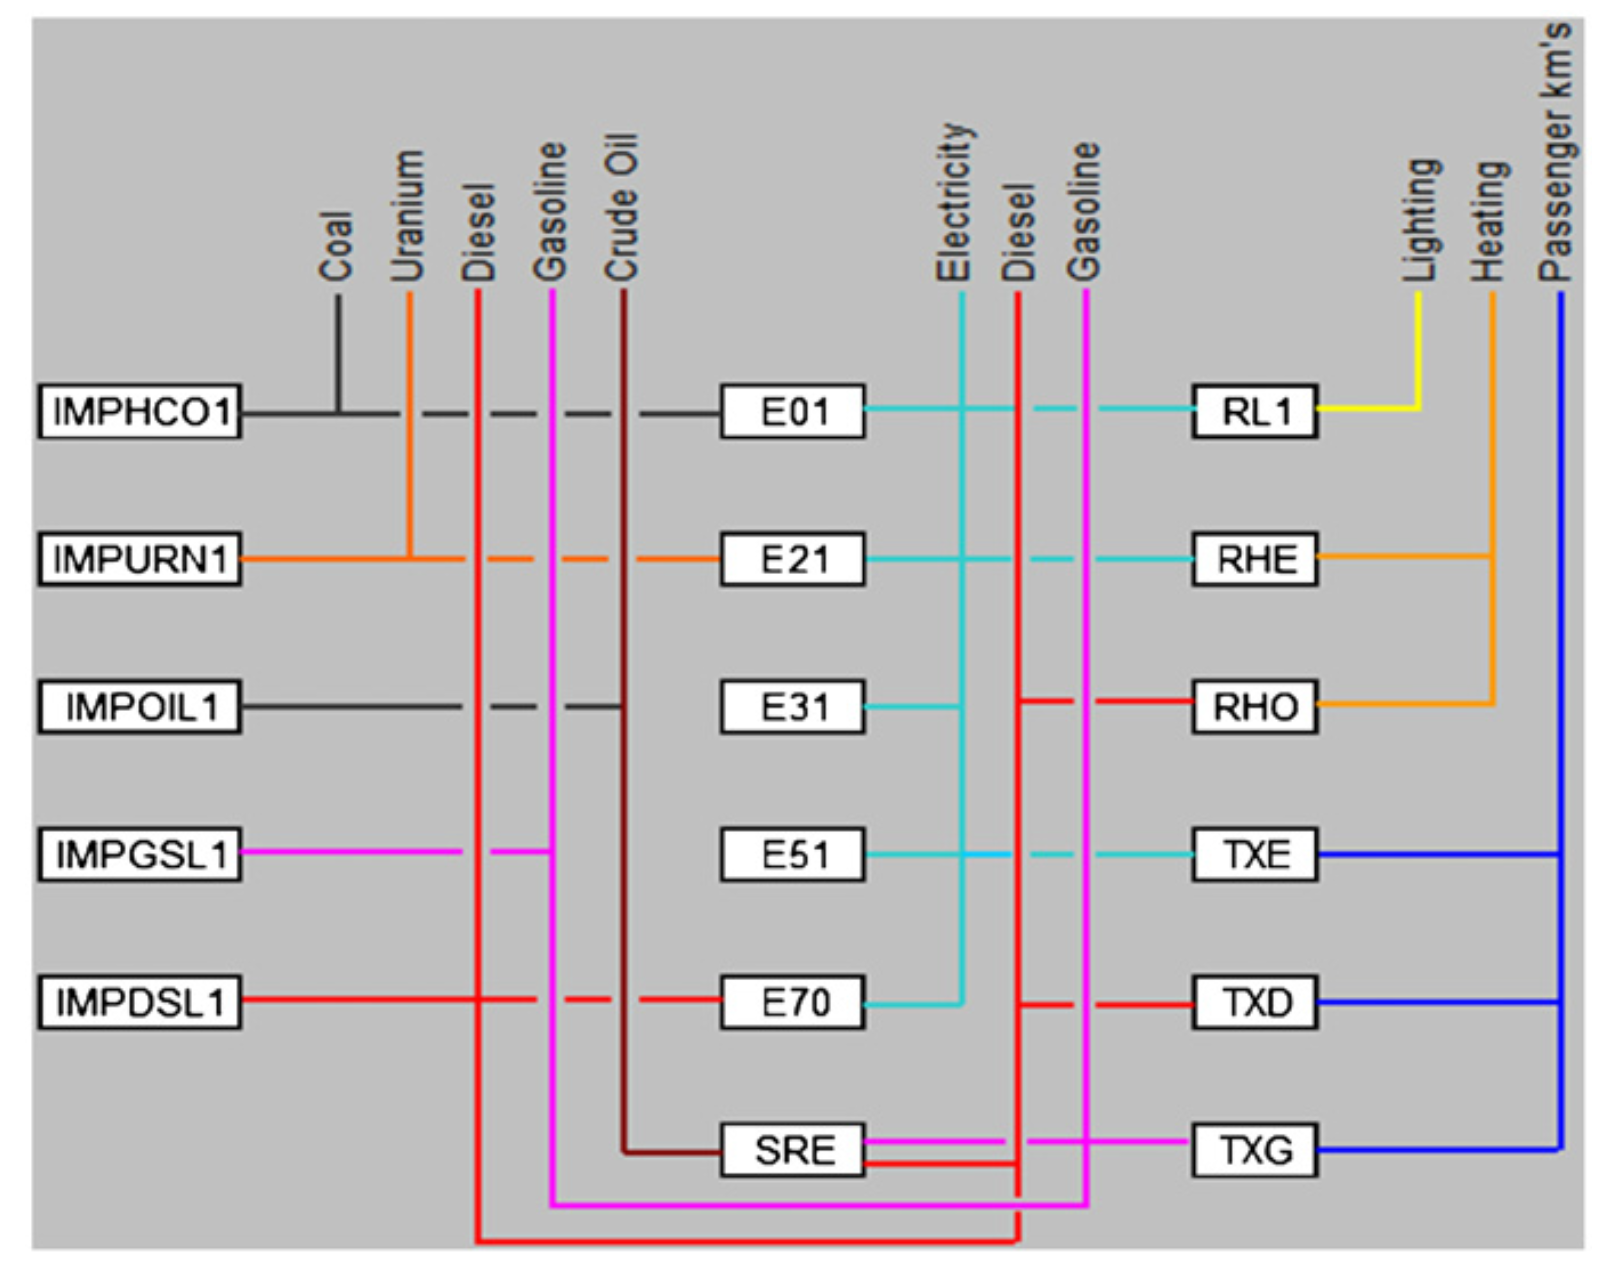
\includegraphics[width=0.8\textwidth]{RES}
    \caption{Reference Energy System (RES) structure of the OSeMOSYS model.}
    \label{fig:osemosys_structure}
\end{figure}

\subsection{Parameters}
Below are the parameters that are predefined in the model based on the assumptions.

\subsubsection{Cost}
\begin{itemize}
    \item $VariableCost(y,t,m,r)$: The per-unit cost of operating technology t in year y, mode m, and region r (in \$/PJ).
    \item $FixedCost(y,t,r)$: The fixed cost of technology t in year y and region r (in \$/PJ/year).
    \item $DiscountRate(t,r)$: The discount rate to convert technology t in region r to net value (as a decimal).
    \item $CapitalCost(y,t,r)$: The capital cost of building one unit of technology t in year y and region r (in \$/PJ).
    \item $OperationalLife(t,r)$: The operational life of technology t in region r (in years).
\end{itemize}


\subsection{Storage}
\begin{itemize}
    \item $TechnologyToStorage(t,m,s,r)$: The conversion factor for technology t in mode m and region r to charge per unit.
    \item $TechnologyFromStorage(t,m,s,r)$: The conversion factor for technology t in mode m and region r to discharge per unit.
    \item $YearSplit(y,l)$: The fraction of year y represented by timeslice l (as a decimal).
    \item $StorageInflectionTimes(y,l,b)$: The fraction of year y represented by timeslice l on daytype b (as a decimal).
    \item $StorageLowerLimit(s,r)$: The minimum storage level for storage technology s in region r (in PJ).
    \item $StorageUpperLimit(s,r)$: The maximum storage level for storage technology s in region r (in PJ).
\end{itemize}

\subsection{Capacity}
\begin{itemize}
    \item $ResidualCapacity(t,r)$: The existing capacity of technology t in region r at the start of the model (in PJ year).
    \item $CapacityFactor(y,t,r)$: The capacity factor of technology t in year y and region r (as a decimal).
    \item $CapacityToActivityUnit(t,r)$: The conversion factor from capacity to activity for technology t in region r (in PJ/year).
\end{itemize}


\subsection{Technology Performance}
\begin{itemize}
    \item $OutputActivityRatio(y,t,f,m,r)$: The output activity ratio of technology t in year y, fuel f, mode m, and region r.
    \item $InputActivityRatio(y,t,f,m,r)$: The input activity ratio of technology t in year y, fuel f, mode m, and region r.
\end{itemize}

\subsection{Demand}
\begin{itemize}
    \item $AccumulatedAnnualDemand(y,t,r)$: The accumulated annual demand for technology t in year y and region r (in MWh).
\end{itemize}

\subsection{Capacity and Activity Limits}
\begin{itemize}
    \item $TotalAnnualMaxCapacity(y,t,r)$: The total annual maximum capacity for technology t in year y and region r (in MW).
    \item $TotalAnnualMaxCapacityInvestment(y,t,r)$: The total annual maximum capacity investment for technology t in year y and region r (in MW).
    \item $TotalTechnologyAnnualActivityUpperLimit(y,t,r)$: The total technology annual activity upper limit for technology t in year y and region r (in MWh).
    \item $TotalTechnologyAnnualActivityLowerLimit(y,t,r)$: The total technology annual activity lower limit for technology t in year y and region r (in MWh).
    \item $TotalTechnologyModelPeriodActivityUpperLimit(t,r)$: The total technology model period activity upper limit for technology t in region r (in MWh).
    \item $TotalTechnologyModelPeriodActivityLowerLimit(t,r)$: The total technology model period activity lower limit for technology t in region r (in MWh).
\end{itemize}

\subsection{Reserve Margin}
\begin{itemize}
    \item $ReserveMarginTagTechnology(y,t,r)$: The fraction of reserve margin for technology t in year y and region r to contribute to meet the margin (as a decimal).
    \item $ReserveMarginTagFuel(y,f,r)$: The fraction of reserve margin for fuel f in year y and region r to contribute to meet the margin (as a decimal).
    \item $ReserveMargin(y,r)$: The required fraction of reserve margin for year y and region r (as a decimal).
\end{itemize}

\subsection{Emissions}
\begin{itemize}
    \item $EmissionActivityRatio(y,t,m,e,r)$: The fraction of emissions for technology t in year y, mode m, and region r (as a decimal).
    \item $EmissionPenalty(y,e,r)$: The emission intensity for technology t in year y, mode m, and region r (as a decimal).
    \item $AnnualExogenousEmission(y,e,r)$: The total annual emissions for region r in year y for emission type e (in tCO2, tNOx).
    \item $ModelPeriodExogenousEmission(e,r)$: The total model period emissions for region r for emission type e (in tCO2, tNOx).
    \item $AnnualEmissionLimit(y,e,r)$: The annual emission limit for region r in year y for emission type e (in tCO2, tNOx).
    \item $ModelPeriodEmissionLimit(e,r)$: The model period emission limit for region r for emission type e (in tCO2, tNOx).
\end{itemize}

\subsection{Implementation}
I am using an open-source implementation of OSeMOSYS in github \cite{githubrepo} that is written in Python. The implementation uses the PuLP library to define and solve the optimization model.

\subsection{Verification and Testing}
There is not real verification as the real-world scenarios does not necessarily follow the minimized cost this model aims to achieve. However, I want to use the published data from 2010 to 2020 to see how well the model can predict the energy system's behavior during this period. I will compare the model's output with the actual data to assess its accuracy and reliability.


\section{Accumplished Work}
\subsection{Model Setup}
I have successfully set up the OSeMOSYS model using the open-source implementation in Python. I have defined the model's parameters, variables, and constraints based on the assumptions and objectives outlined in the background section.

\subsection{Visualization}
The model itself does not have a built-in visualization tool. However, I have created some visualizations using Python libraries such as Matplotlib to help analyze and interpret the model's output. For example, I have created plots showing the Total Capacity by Technology over the years, as shown in Figure \ref{fig:total_capacity}, Total Technology Capacity over time, as shown in Figure \ref{fig:total_technology_capacity}.
\begin{figure}[H]
    \centering
    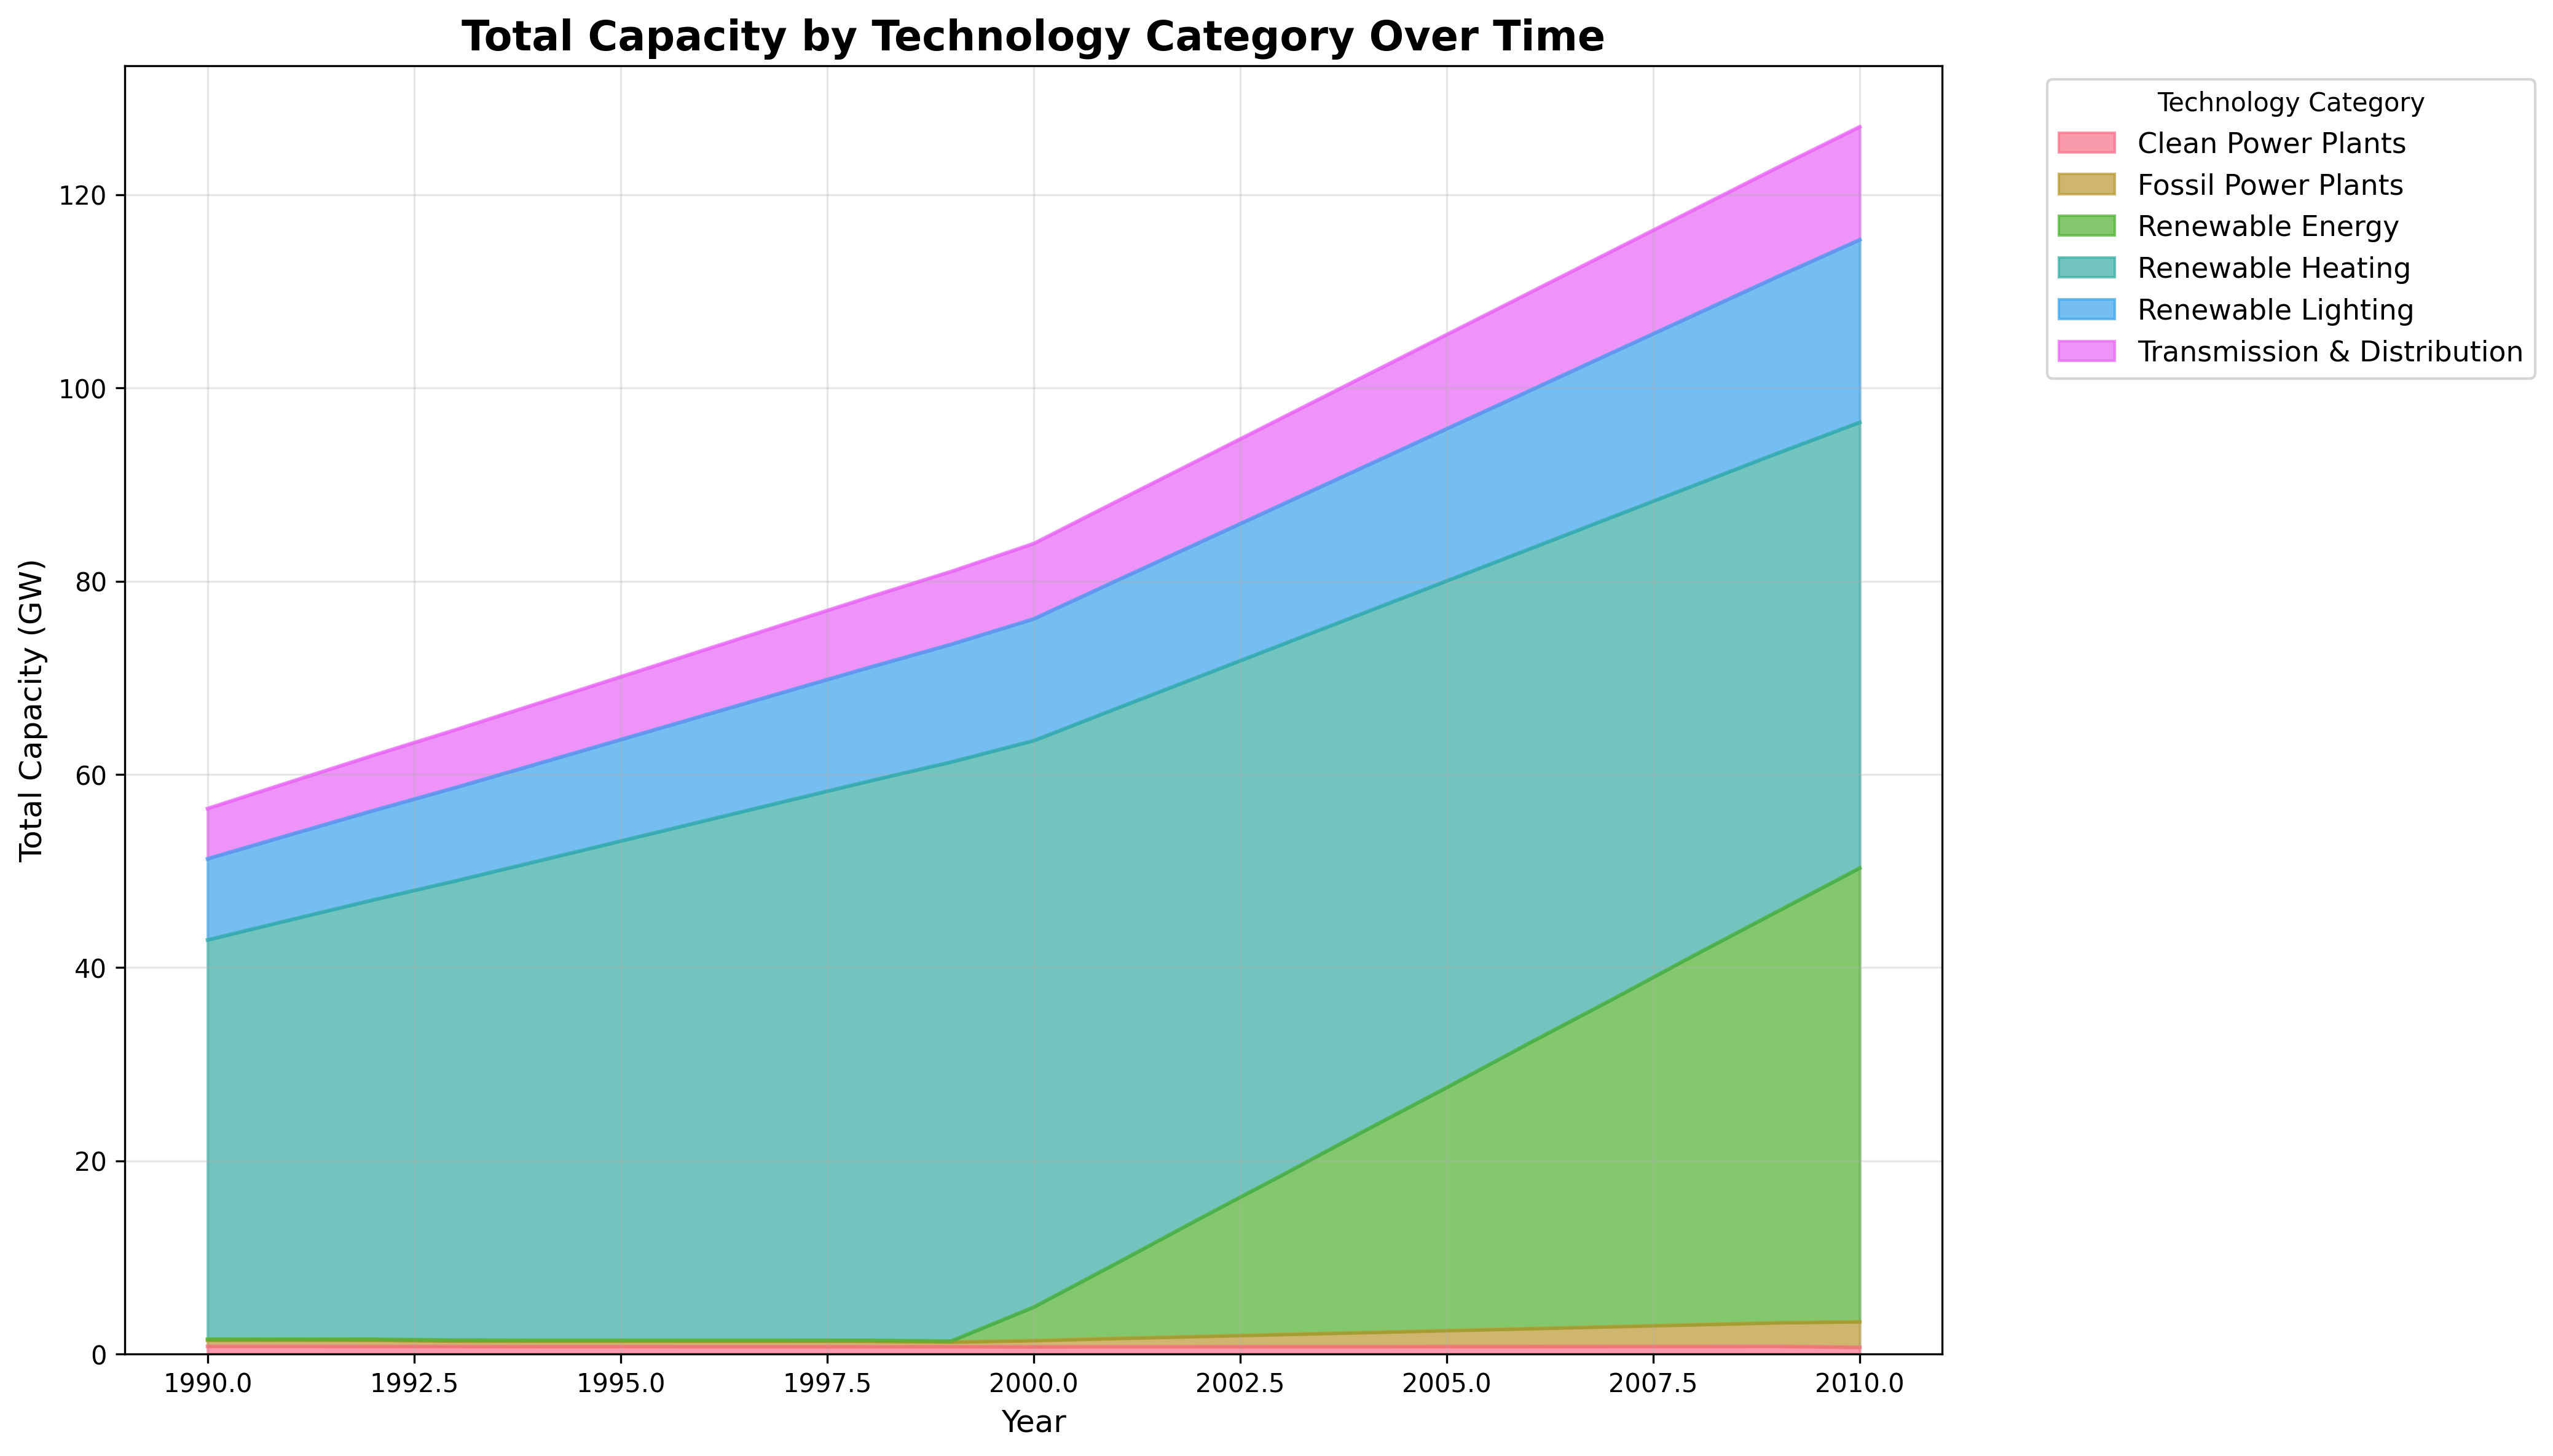
\includegraphics[width=0.8\textwidth]{capacity_by_category_labeled.png}
    \caption{Total Capacity by Technology over the years.}
    \label{fig:total_capacity}
\end{figure}

\begin{figure}[H]
    \centering
    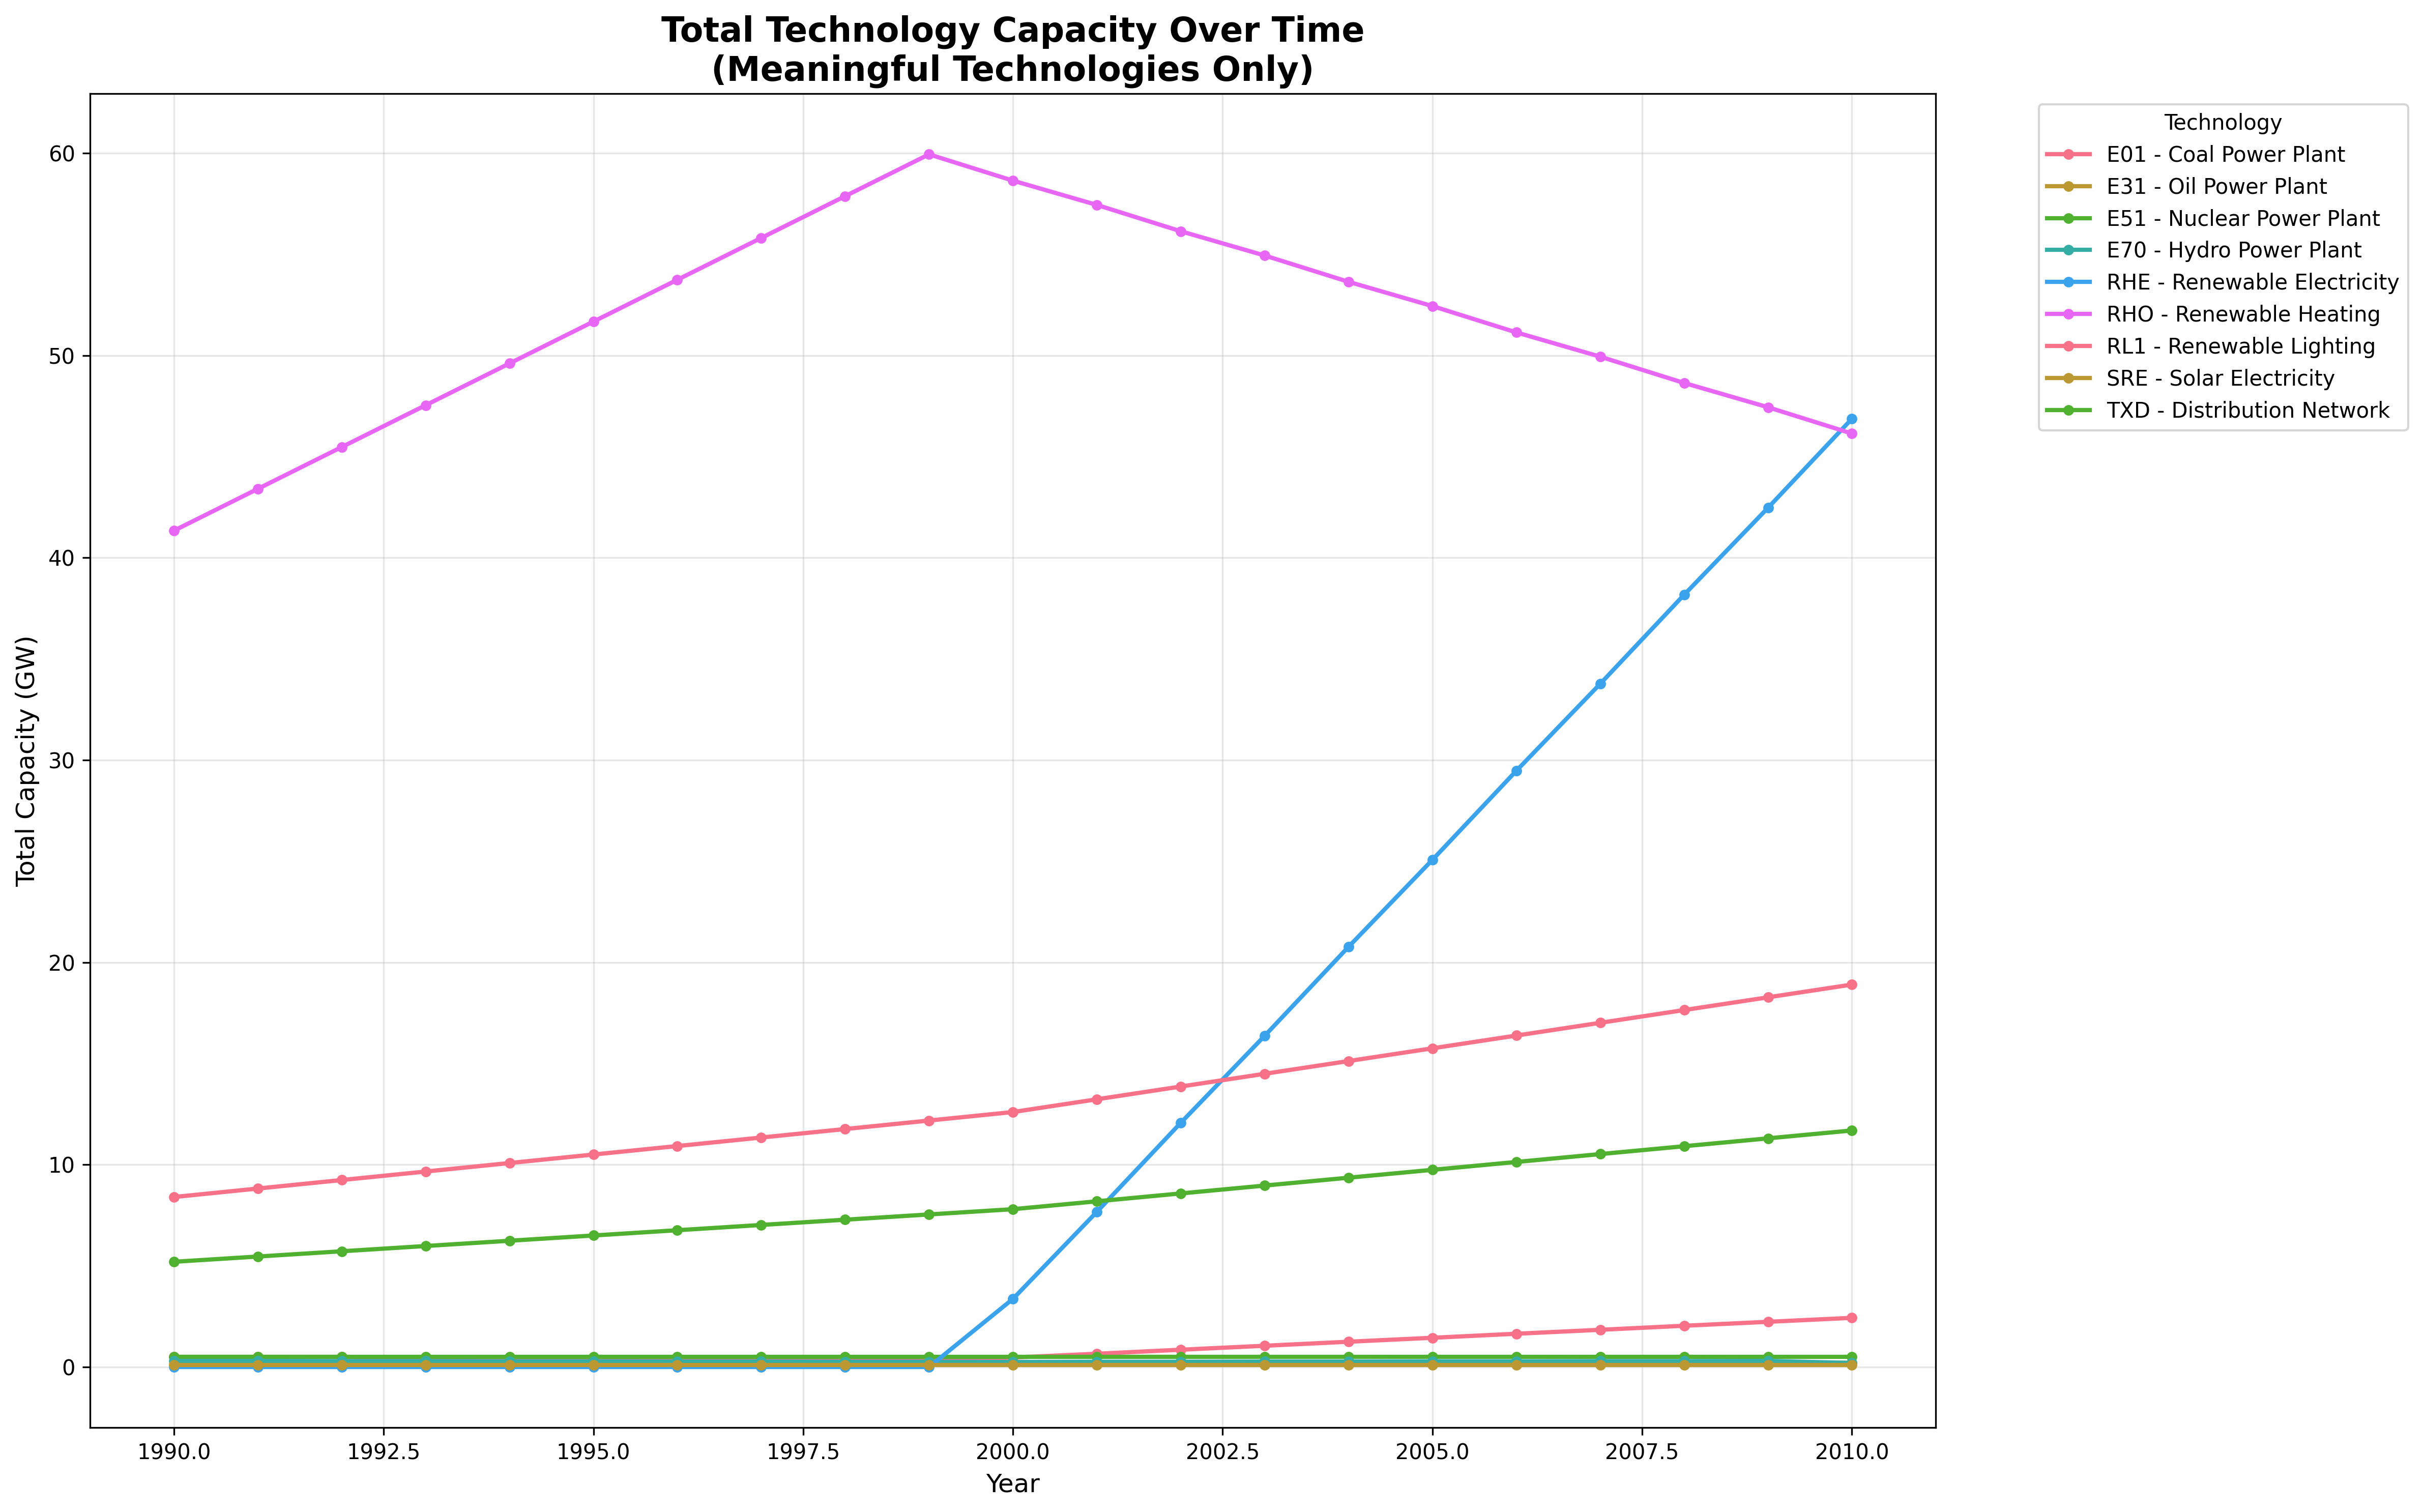
\includegraphics[width=0.8\textwidth]{meaningful_total_capacity_labeled.png}
    \caption{Total Technology Capacity over time.}
    \label{fig:total_technology_capacity}
\end{figure}

As for the optimized result, I have created the New Technology Investment over time, as shown in Figure \ref{fig:new_technology_investment}.
\begin{figure}[H]
    \centering
    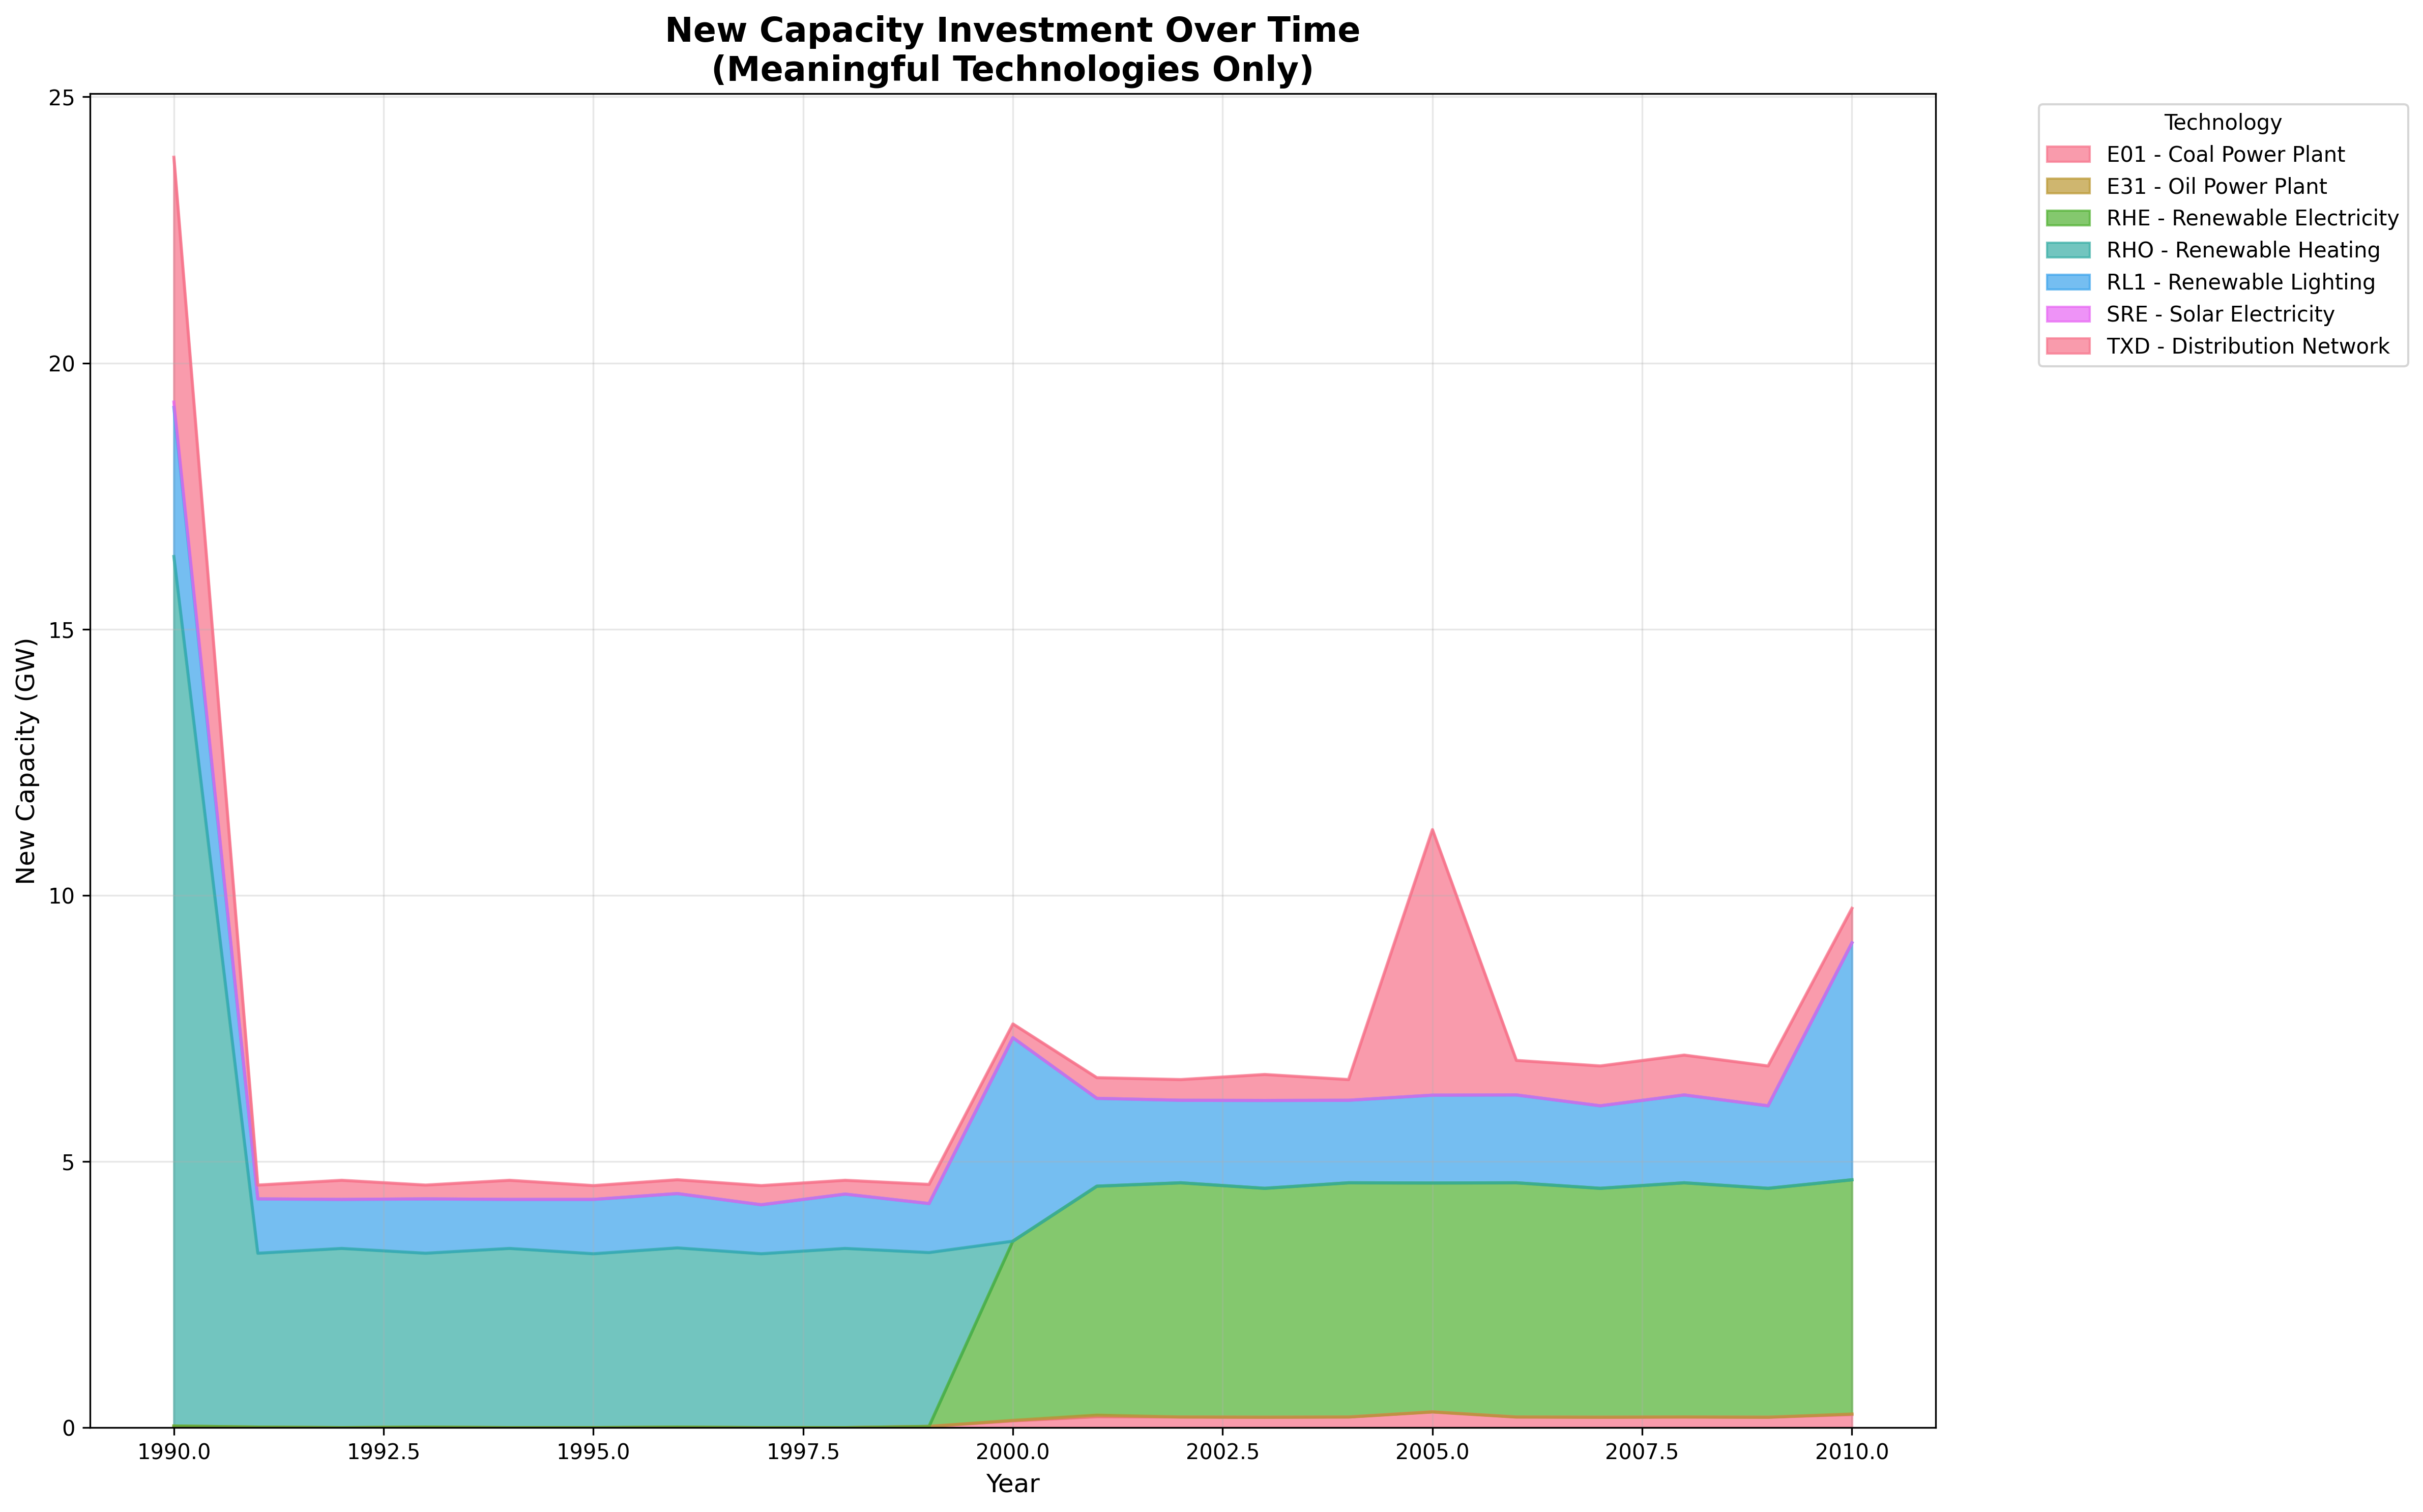
\includegraphics[width=0.8\textwidth]{meaningful_technology_capacity_labeled.png}
    \caption{New Technology Investment over time.}
    \label{fig:new_technology_investment}
\end{figure}    

\section{Remaining Work}
\subsection{Model Enhancement}
I plan to enhance the model by incorporating additional features and functionalities. This may include adding charge and discharge efficiencies for storage technologies, mimicking policy interventions that affect the technology costs, creating comprehensive testing and visualization functionalities. At the same time, I would like to collect real-world data to compare the model's predictions with actual outcomes.

\section{Potential Challenges}
Some potential challenges I anticipate include:
\begin{itemize}
    \item Data Availability: Accessing high-quality, real-world data for model validation may be difficult.
    \item Model Complexity: As I add more features and functionalities, the model may become more complex and harder to solve.
    \item Computational Resources: The optimization process may require significant computational resources, especially for large-scale models.
\end{itemize}


\bibliographystyle{plain}
\bibliography{references}

\end{document}